\documentclass[11pt]{article}

\usepackage{amsmath, amssymb, amscd, amsthm, amsfonts}
\usepackage{graphicx}
\usepackage{hyperref}
\usepackage{caption}
\captionsetup[figure]{font=small}
%\addbibresource{NWUSForestVirome.bib}

\title{A very cool project to start}
\author{Ricardo I. Alcal\'a-Brse\~no}
\date{}

\begin{document}

\maketitle

\begin{abstract}
Viruses plays different roles in plant ecosystems, and viruses are cool, that's why we studied them.   
\end{abstract}

\section{Introduction}\label{section-introduction}
	
The study of viruses started by characterizing tobacco mosaic virus, genus {\it Tobamovirus}, family {\it Virgaviridae} in tobacco plants. Since then, thousands of virus species have been described in plants and other organisms such as fungi and oomycetes, including other phyla, and not to mention other domains \cite{roossinck_viruses_2019, dolja_deep_2020}. 
However, very little is known about the diversity of viruses in the United States, and virus epidemics are understudied in the world.

\section{Background}
\subsection{Viral Isolation}
Extraction methods are specific for each group of viruses. These techniques can target naked viruses, such {\it Amalgavirus} and {\it Endornavirus}, which are double-stranded RNA viruses \cite{alcala2017genome, alcala2018novel}. Other methods target viruses surrounded by capsid proteins (encapsidated), either single-stranded RNA genomes, which are most plant viruses. And circular DNA viruses, single-stranded genomes in the families {\it Geminviridae} and {\it Nanoviridae} \cite{boukari2017occurrence}, and double-stranded DNA viruses in the {\it Caulimoviridae} family –or pararetroviruses– some genera in this family can integrate into the host genome \cite{saad2020blueberry}. 

The most common method for virus sequencing is Illumina, constructing RNA or DNA libraries for single or paired-end reads (I prefer PE X 150 or 250 nt) \cite{alcala2017genome, alcala2018novel, alcala2020network}. I can implement standard methods for determining read quality, and tag removal can be used. However, some sequencing results yield double-stranded nucleic acids that are expected due to the nature of the purification methods. Part of the sequence filtering is implemented in the bioinformatic pipeline.

\subsection{Viral Metagenomics}
The implementation of viral metagenomics allows the characterization of viruses using high-throughput sequencing approaches and bioinformatic tools \cite{roossinck_metagenomics_2015, roossinck_plant_2015}. Several approaches to sequence viruses have been implemented by bulking samples of different species and sequence them (plant metagenomics) to several species from ecological and agricultural importance sampled in bulks (agroeco-genomics) and individual hosts (eco-genomics) \cite{roossinck_plant_2015}.  
Several viral assembly pipelines have been developed and tested for virus identification \cite{doi:10.1094/PHYTO-02-18-0067-R}. Most programs perform well for abundant viruses, and a couple of software are more sensitive to less abundant species . Several custom pipelines can be implemented according to the virome characteristic and research needs. For example, in the papaya orchard virome \cite{alcala2020network}, a full-length genome was the minimum threshold to count for a virus species. Other approaches consist in assigning viral operational taxonomic units (vOTUs) to assign viral categories \cite{doi:10.1094/PBIOMES-07-19-0037-A}, or others that implement semi-supervised machine learning that assigns species according to the International Committee for the Taxonomy of Viruses (ICTV) demarcation criteria of virus species  (Alcal\'a-Brise\~no et al., manuscript in prep). 

\subsection{Virus Characterization and Taxonomy}
The plant samples processed with HTS and bioinformatic pipelines help to identify viruses present in the host. The virus identified can be represented as a super contig representing a full-length virus genome or multiple contigs that can be scaffolded to generate a full-length virus genome. However, multiple contigs often corresponding to a virus species can not generate a full length and are represented as partial sequences that are usually problematic to classify (Fig 1).

\begin{figure}[h!]
\centerline{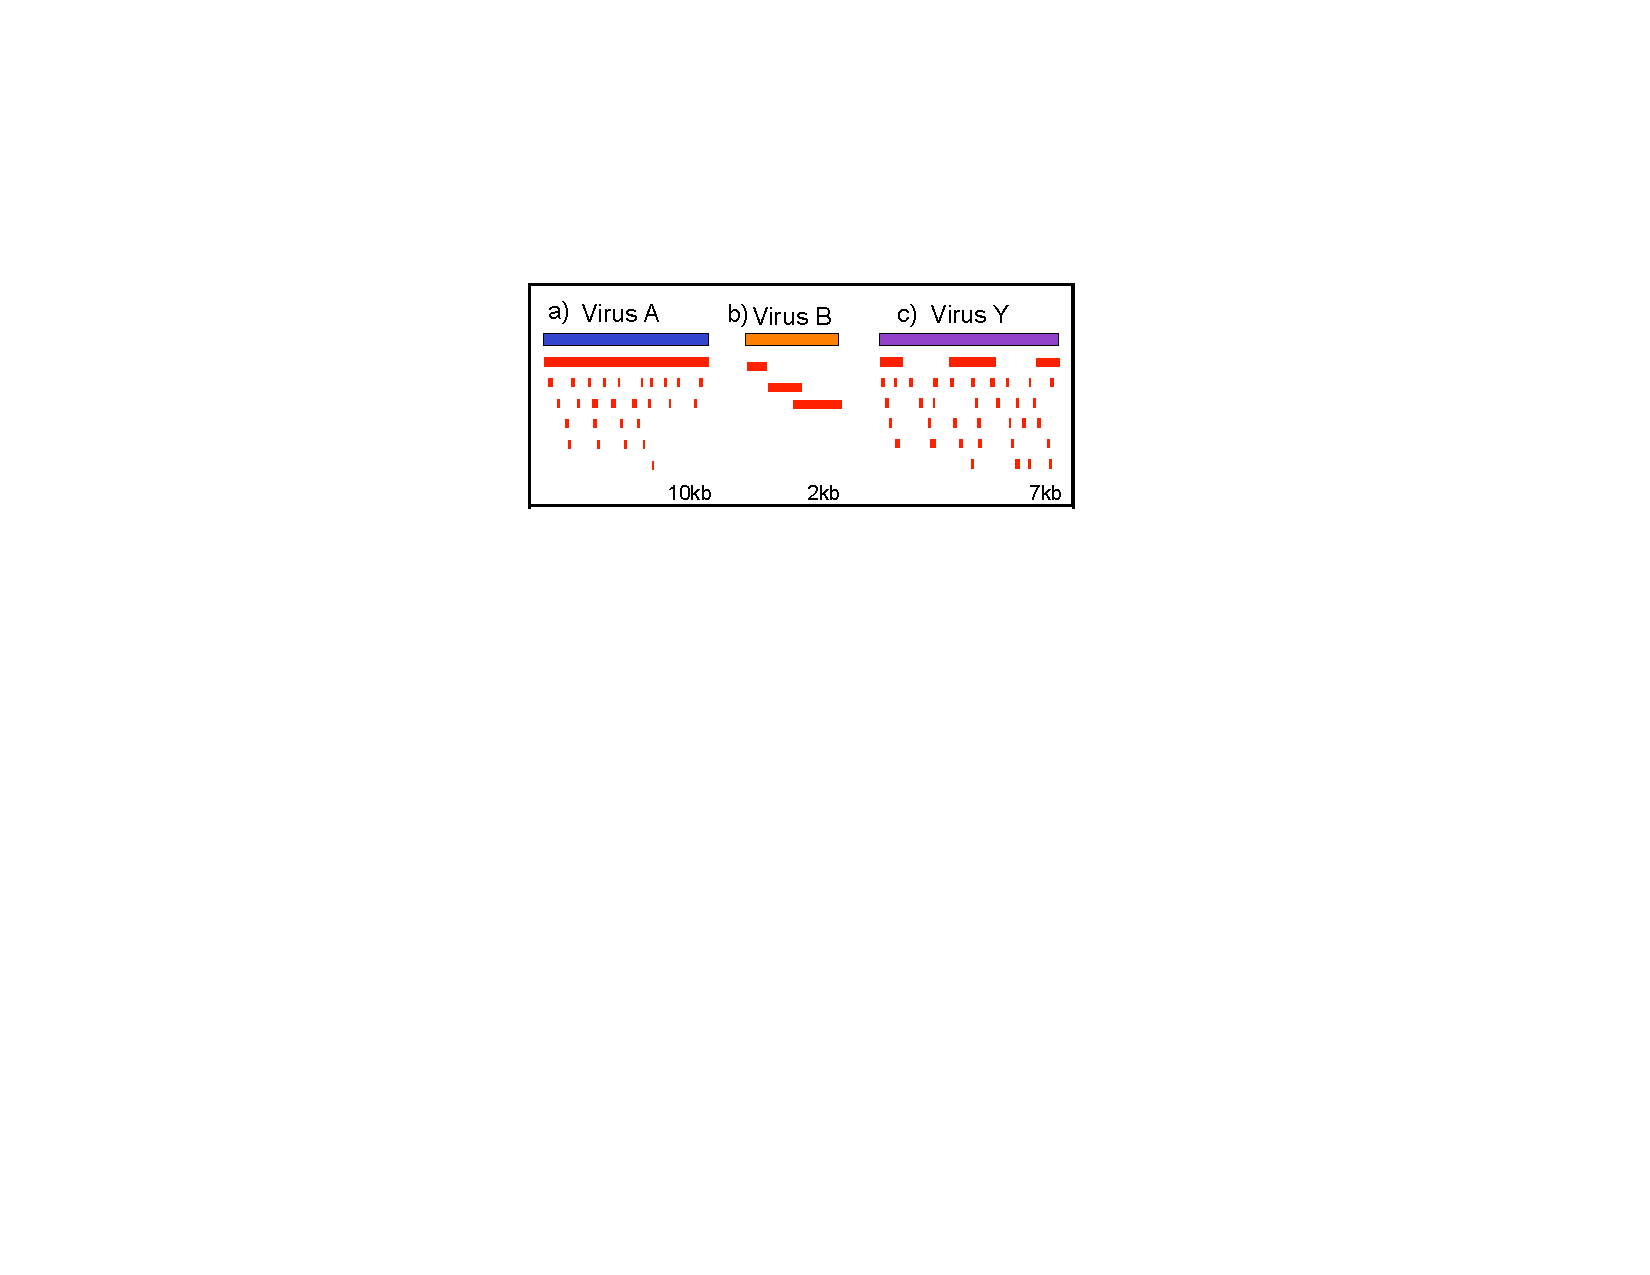
\includegraphics[scale=1]{figs/Fig3_contigs.pdf}}
\caption{An example of contigs partition. a) Super contig assembled, b) several contigs assembled allowing to generate a scaffold, c) several contigs that does not allow to generate a scaffold}
\end{figure}

Fortunately, characterizing full-length genome sequences of viruses is relatively straightforward. Most methods utilize BLAST searches to identify sequences homology to viruses, narrowing it down to one of the ~65 plant virus genera described till now \cite{king_virus_2011, lefkowitz_virus_2018}. Using sequence data, the ICTV determines the virus species demarcation criteria based on pairwise similarities and/or phylogenetics using sequence data \cite{lefkowitz_virus_2018}. However, other physicochemical and biological characteristics are considered \cite{king_virus_2011, lefkowitz_virus_2018} 
Genome and gene phylogenetic relationship dictates virus taxonomical classification for species, genus, family, and order. Until recently, that virus classification was updated to seven realms \cite{gorbalenya_new_2020}. 

\bibliographystyle{acm}
\bibliography{bibliography}  	% see references.bib for bibliography management

\end{document}
